\documentclass[11pt,a4paper]{article}
\usepackage[margin=2.4cm]{geometry}
\usepackage{amsmath,amssymb}
\usepackage{graphicx}
\usepackage{booktabs}
\usepackage{listings}
\usepackage{xcolor}
\usepackage[colorlinks=true,linkcolor=blue!50!black,citecolor=blue!50!black,urlcolor=blue!50!black]{hyperref}
\usepackage{natbib}
\lstset{basicstyle=\ttfamily\scriptsize,columns=fullflexible,breaklines=true,
        frame=single,rulecolor=\color{gray!50},keywordstyle=\color{blue!60!black},
        commentstyle=\color{green!40!black},language=Python,showstringspaces=false}
\newcommand{\dd}{\mathrm{d}}
\newcommand{\Rb}{R_b}
\newcommand{\md}{\langle\delta\rangle}

\title{Two pictures of one top hat\\[4pt]
\large The shell equation, the nonlinear equation for $\delta$, and the mean
density of our seed\\[2pt]
\normalsize A companion note to \emph{From a primordial fluctuation to an idealised rotation curve}}
\author{B. R. Parodi}
\date{24 October 2026}

\begin{document}
\maketitle

\begin{abstract}
The collapse of a uniform overdense sphere, the \emph{top hat}, can be
described in two ways: by Newton's equation for the radius of its edge,
or by a nonlinear differential equation for its density contrast
$\delta$, the form used in most papers on spherical collapse in
dark-energy cosmologies. We show step by step that the two are the same
equation, that the cosmological constant drops out of the equation for
$\delta$ because it acts on the sphere exactly as on the background, and
that the cycloid of our main paper is the exact solution of the
$\delta$ equation in an Einstein--de Sitter universe. The mean
overdensity inside each shell of our seed is therefore a solution of the
nonlinear $\delta$ equation, one for every shell: the seed is a family
of nested top hats, which share one solution shifted in time. We give
the closed form, its linear limit and its values at turnaround
($1+\md=5.55$), halting (147) and collapse ($\infty$), verify the
equivalence numerically in a flat $\Lambda$CDM background to better than
$10^{-6}$, and state where the $\delta$ picture ends: at shell crossing,
which in our model begins at the halting front.
\end{abstract}

\section{Why two pictures?}

A spherical region that is slightly denser than its surroundings expands
more slowly than the Universe, stops, and falls back. If the region is
uniform, a top hat, it behaves as a small closed universe of its own
\citep{Gunn1972,Peebles1980}. Two descriptions are in use:
\begin{itemize}
\item the \textbf{shell (or radius) picture}: follow the radius $R(t)$ of
the edge of the sphere, which encloses a fixed mass $M$ and obeys
Newton's law. This is what our main paper does, shell by shell;
\item the \textbf{density picture}: follow the density contrast
$\delta(t)=\rho/\bar\rho-1$ of the sphere relative to the background. This
is the language of cosmological perturbation theory, and the one in
which spherical collapse is extended to dark energy, modified gravity,
shear and rotation
\citep[e.g.][]{Fosalba1998,DelPopolo2013,Herrera2019}.
\end{itemize}
The second picture produces an equation that looks complicated,
\begin{equation}
  \ddot\delta+2H\dot\delta-\frac43\,\frac{\dot\delta^{2}}{1+\delta}
  =4\pi G\bar\rho\,\delta(1+\delta)
  =\frac32\,H^{2}\Omega_{\rm m}(t)\,\delta(1+\delta),
  \label{eq:delta}
\end{equation}
where $H=\dot a/a$ is the Hubble rate, $\bar\rho$ the mean matter density
of the background and $\Omega_{\rm m}(t)=8\pi G\bar\rho/3H^{2}$. It is
eq.~(10) of \citet{Herrera2019} for a cosmological constant (their
$\gamma=1$, $\delta_{\rm de}=0$), and the starting point of many papers.
The aim of this note is to show that Eq.~\eqref{eq:delta} contains
nothing that is not already in the shell equation of our paper, and to
see what this means for our seed.

\section{The shell picture}

A shell of mass $M$ at radius $R$ is pulled by the mass inside it and,
in the presence of a cosmological constant $\Lambda$ (in units of
$1/\text{time}^{2}$), pushed outward by $\Lambda R/3$:
\begin{equation}
  \ddot R=-\frac{GM}{R^{2}}+\frac{\Lambda}{3}\,R .
  \label{eq:shell}
\end{equation}
As long as no other shell crosses it, $M$ is constant. Multiplying by
$\dot R$ and integrating gives the conserved specific energy
\begin{equation}
  E=\frac12\dot R^{2}-\frac{GM}{R}-\frac{\Lambda}{6}R^{2}.
  \label{eq:energy}
\end{equation}
For $\Lambda=0$ and $E<0$ the solution is the cycloid
\begin{equation}
  R=A(1-\cos\eta),\qquad t=B(\eta-\sin\eta),\qquad
  A=\frac{GM}{2|E|},\quad B=\frac{GM}{(2|E|)^{3/2}},
  \label{eq:cycloid}
\end{equation}
which reaches its maximum, \emph{turnaround}, $R_{\rm ta}=2A$, at
$\eta=\pi$, and collapses to a point at $\eta=2\pi$. Note the identity
\begin{equation}
  \frac{A^{3}}{B^{2}}=GM ,
  \label{eq:AB}
\end{equation}
which follows directly from the definitions of $A$ and $B$ and will make
the mass drop out below.

The background obeys the same kind of equation. A sphere of the
\emph{unperturbed} Universe of comoving radius $X$ has physical radius
$aX$, and the Friedmann equations for matter and $\Lambda$ read
\begin{equation}
  \frac{\ddot a}{a}=-\frac{4\pi G}{3}\bar\rho+\frac{\Lambda}{3},\qquad
  H^{2}=\frac{8\pi G}{3}\bar\rho+\frac{\Lambda}{3},\qquad
  \bar\rho\,a^{3}=\text{const}.
  \label{eq:friedmann}
\end{equation}
In words: the background is itself a family of shells, each obeying
Eq.~\eqref{eq:shell} with the mean density inside it. The top hat
differs from the background only in that it contains more mass for its
size.

\section{From the shell to the density contrast}\label{sec:derivation}

The mean density inside the shell is $\rho=3M/(4\pi R^{3})$. Divided by
the background density, and using $\bar\rho a^{3}=$ const,
\begin{equation}
  1+\delta=\frac{\rho}{\bar\rho}=K\,\Bigl(\frac{a}{R}\Bigr)^{3},
  \qquad K=\text{const}.
  \label{eq:oneplusdelta}
\end{equation}
\emph{The density contrast is nothing but the cube of the ratio of two
radii}: that of a background sphere, which grows as $a$, and that of the
shell, $R$. Everything else follows by differentiating twice.

\paragraph{First derivative.} Take the logarithm of
Eq.~\eqref{eq:oneplusdelta}, $\ln(1+\delta)=\ln K+3\ln a-3\ln R$, and
differentiate with respect to time. With $h\equiv\dot R/R$, the local
expansion rate of the shell,
\begin{equation}
  \frac{\dot\delta}{1+\delta}=3\,(H-h)
  \qquad\Longleftrightarrow\qquad
  h=H-\frac{\dot\delta}{3(1+\delta)} .
  \label{eq:first}
\end{equation}
The contrast grows exactly when the shell expands more slowly than the
background. This is also the continuity equation of a uniform fluid
sphere: $\dot\rho/\rho=-3h$ and $\dot{\bar\rho}/\bar\rho=-3H$.

\paragraph{Second derivative.} Differentiate Eq.~\eqref{eq:first} once
more:
\begin{equation}
  \frac{\ddot\delta}{1+\delta}-\frac{\dot\delta^{2}}{(1+\delta)^{2}}
  =3\,(\dot H-\dot h).
  \label{eq:second}
\end{equation}
For any scale factor, $\dot H=\ddot a/a-H^{2}$, and likewise
$\dot h=\ddot R/R-h^{2}$. Hence
\begin{equation}
  \dot H-\dot h=\Bigl(\frac{\ddot a}{a}-\frac{\ddot R}{R}\Bigr)-(H^{2}-h^{2}).
  \label{eq:split}
\end{equation}
The first bracket contains the forces, the second the kinematics.

\paragraph{The forces: $\Lambda$ cancels.} From Eqs.~\eqref{eq:shell}
and \eqref{eq:friedmann},
\begin{equation}
  \frac{\ddot a}{a}-\frac{\ddot R}{R}
  =\Bigl(-\frac{4\pi G}{3}\bar\rho+\frac{\Lambda}{3}\Bigr)
   -\Bigl(-\frac{GM}{R^{3}}+\frac{\Lambda}{3}\Bigr)
  =\frac{4\pi G}{3}\,(\rho-\bar\rho)
  =\frac{4\pi G}{3}\,\bar\rho\,\delta .
  \label{eq:forces}
\end{equation}
This is the heart of the matter. The cosmological constant produces an
acceleration proportional to distance, $\Lambda R/3$, so it stretches the
shell and the background at exactly the same rate and drops out of their
\emph{difference}. Only the excess of matter, $\rho-\bar\rho$, drives the
contrast. This is why $\Lambda$ ``cannot cluster'': in the language of
\citet{Herrera2019}, the cosmological constant has $\delta_{\rm de}=0$
for every top hat. It still enters Eq.~\eqref{eq:delta}, but only through
the background, i.e.\ through $H(t)$ and $\Omega_{\rm m}(t)$.

\paragraph{The kinematics.} With Eq.~\eqref{eq:first},
$H-h=\dot\delta/[3(1+\delta)]$ and
$H+h=2H-\dot\delta/[3(1+\delta)]$, so
\begin{equation}
  3\,(H^{2}-h^{2})=3(H-h)(H+h)
  =\frac{2H\dot\delta}{1+\delta}-\frac{\dot\delta^{2}}{3(1+\delta)^{2}} .
  \label{eq:kin}
\end{equation}

\paragraph{Putting it together.} Inserting Eqs.~\eqref{eq:forces} and
\eqref{eq:kin} into Eqs.~\eqref{eq:split} and \eqref{eq:second},
\begin{equation*}
  \frac{\ddot\delta}{1+\delta}-\frac{\dot\delta^{2}}{(1+\delta)^{2}}
  =4\pi G\bar\rho\,\delta-\frac{2H\dot\delta}{1+\delta}
  +\frac{\dot\delta^{2}}{3(1+\delta)^{2}},
\end{equation*}
and multiplying by $1+\delta$ gives exactly Eq.~\eqref{eq:delta}:
\begin{equation*}
  \ddot\delta+2H\dot\delta-\frac43\,\frac{\dot\delta^{2}}{1+\delta}
  =4\pi G\bar\rho\,\delta(1+\delta).
\end{equation*}
Each term now has a plain meaning. $2H\dot\delta$ is the \emph{Hubble
drag}: the expanding background dilutes the growth. The term
$\frac43\dot\delta^{2}/(1+\delta)$ is purely kinematic; it comes from
writing a ratio of volumes, Eq.~\eqref{eq:oneplusdelta}, as a contrast,
and it is what makes the growth run away once $\delta\gtrsim1$. The right-hand
side is the gravitational pull of the excess mass, $\bar\rho\delta$,
enhanced by the factor $1+\delta$ because the sphere has shrunk relative
to the background.

\paragraph{The fluid route, and where shear and rotation enter.} The same
equation follows from the continuity, Euler and Poisson equations of a
pressureless fluid. Taking the divergence of the Euler equation gives
the Raychaudhuri equation for the expansion $\theta=\nabla\cdot\mathbf u$,
which contains the shear $\sigma^{2}$ and the vorticity $\omega^{2}$ of the
flow; the result is Eq.~\eqref{eq:delta} with an extra term
$-(1+\delta)(\sigma^{2}-\omega^{2})$ on the left
\citep{Fosalba1998,DelPopolo2013}. For a top hat both vanish: a uniform
sphere expanding or contracting radially is neither sheared nor rotated.
Models that keep $\sigma^{2}-\omega^{2}$ go beyond the top hat; in the shell
picture the rotation corresponds to a centrifugal term $j^{2}/R^{3}$ in
Eq.~\eqref{eq:shell}, which our main paper adds to each shell only after
its turnaround.

\section{The exact solution: the cycloid}\label{sec:cycloid}

Without $\Lambda$, in an Einstein--de Sitter (EdS) background,
$\bar\rho=1/(6\pi Gt^{2})$, $H=2/(3t)$ and $\Omega_{\rm m}=1$. With the
cycloid~\eqref{eq:cycloid} and the identity~\eqref{eq:AB},
\begin{equation}
  1+\md=\frac{3M}{4\pi A^{3}(1-\cos\eta)^{3}}\;6\pi G B^{2}(\eta-\sin\eta)^{2}
  =\frac92\,\frac{GMB^{2}}{A^{3}}\,\frac{(\eta-\sin\eta)^{2}}{(1-\cos\eta)^{3}}
  =\frac92\,\frac{(\eta-\sin\eta)^{2}}{(1-\cos\eta)^{3}} .
  \label{eq:exact}
\end{equation}
We write $\md$ for the mean overdensity inside a shell, as in the main
paper. Two remarks:
\begin{itemize}
\item \textbf{The mass and the energy have dropped out.} Every top hat in
EdS runs through the same sequence of $1+\md$ as a function of its
phase $\eta$; only the clock, $t=B(\eta-\sin\eta)$, depends on $M$ and
$E$. Equation~\eqref{eq:delta} in EdS has no scale, so one solution
serves all top hats.
\item \textbf{It is an exact solution.} Equation~\eqref{eq:exact}, read as
a function of $t$ through $t=B(\eta-\sin\eta)$, solves
Eq.~\eqref{eq:delta} identically. Fig.~\ref{fig:tophat}a confirms this
numerically: integrating Eq.~\eqref{eq:delta} from initial values taken
from the cycloid at $\eta=0.05$ reproduces Eq.~\eqref{eq:exact} to
$2\times10^{-8}$ up to $\eta=1.9\pi$.
\end{itemize}

\paragraph{The linear limit.} For small $\eta$,
$\eta-\sin\eta=\frac{\eta^{3}}{6}(1-\frac{\eta^{2}}{20}+\dots)$ and
$1-\cos\eta=\frac{\eta^{2}}{2}(1-\frac{\eta^{2}}{12}+\dots)$, so
\begin{equation}
  1+\md=1+\frac{3}{20}\eta^{2}+O(\eta^{4}),\qquad
  \md\simeq\frac{3}{20}\Bigl(\frac{6t}{B}\Bigr)^{2/3}\propto t^{2/3}\propto a .
  \label{eq:linear}
\end{equation}
This is the growing mode of linear theory. Indeed, dropping the
quadratic terms of Eq.~\eqref{eq:delta} in EdS leaves
$\ddot\delta+\frac{4}{3t}\dot\delta-\frac{2}{3t^{2}}\delta=0$, whose
solutions are $\delta\propto t^{2/3}$ (growing) and $\delta\propto t^{-1}$
(decaying). The cycloid starts on the pure growing mode, the standard
choice; the growing mode solution of \citet[their eq.~19]{Herrera2019},
$\delta_{\rm m}=Ca$, is the same thing.

\paragraph{Milestones.} Table~\ref{tab:milestones} lists the values at
the phases that matter for our model, together with the \emph{linear}
contrast $\delta_{\rm lin}$, i.e.\ Eq.~\eqref{eq:linear} extrapolated to
the same time. The linear value at collapse, $\delta_{\rm c}=1.686$, is
the familiar threshold of the Press--Schechter theory.

\begin{table}[h]
\centering
\caption{Milestones of a top hat in EdS.}
\label{tab:milestones}
\begin{tabular}{lcccc}
\toprule
 & phase $\eta$ & $t/t_{\rm ta}$ & $1+\md$ & $\delta_{\rm lin}$\\
\midrule
turnaround & $\pi$ & 1 & $9\pi^{2}/16=5.55$ & 1.062\\
halting (front) & $3\pi/2$ & $(1+3\pi/2)/\pi=1.82$ & $\frac92(1+3\pi/2)^{2}=146.8$ & 1.583\\
collapse & $2\pi$ & 2 & $\infty$ & 1.686\\
``virialised'' (convention) & -- & 2 & $18\pi^{2}=177.7$ & 1.686\\
\bottomrule
\end{tabular}
\end{table}

The last two rows deserve a comment. In the standard top-hat model the
sphere collapses to a point at $t=2t_{\rm ta}$, which is unphysical; by
convention one assumes it has virialised at half its turnaround radius
by then, which gives $18\pi^{2}\approx178$. Our shells reach the same
radius, $R_{\rm ta}/2$, earlier, at $\eta=3\pi/2$ on their way back
($1-\cos\frac{3\pi}{2}=1$), and halt there. Same radius, earlier time:
the background is denser at $1.82\,t_{\rm ta}$ than at $2t_{\rm ta}$ by
$(2/1.82)^{2}=1.21$, which is exactly the ratio $177.7/146.8$.

\section{With a cosmological constant}\label{sec:lambda}

With $\Lambda>0$ neither Eq.~\eqref{eq:shell} nor Eq.~\eqref{eq:delta}
has a closed-form solution, but they remain the same equation. To check
this numerically, we integrate both in a flat $\Lambda$CDM background
with $\Omega_{\rm m}=0.3$ (units $H_{0}=1$, so $\Lambda=3\Omega_\Lambda
H_{0}^{2}=2.1$), from $a_{\rm i}=1.9\times10^{-3}$ on the growing mode,
for three initial amplitudes (Fig.~\ref{fig:tophat}b): the two
descriptions agree to better than $4\times10^{-7}$ along the whole
evolution.

\paragraph{The turnaround threshold.} The energy~\eqref{eq:energy} shows
what $\Lambda$ changes. The potential $-GM/R-\Lambda R^{2}/6$ has a
maximum at the radius $R_{\Lambda}=(3GM/\Lambda)^{1/3}$, the
\emph{maximum turnaround radius} \citep{Pavlidou2014}. A shell turns
around only if its energy lies below the top of this barrier,
\begin{equation}
  E\le-\frac32\,(GM)^{2/3}\Bigl(\frac{\Lambda}{3}\Bigr)^{1/3};
  \label{eq:threshold}
\end{equation}
for our seed, $E=-v^{2}/2$, this is the condition
$v^{2}\ge3(GM)^{2/3}(\Lambda/3)^{1/3}$ of the main paper (Sect.~3.2),
which bounds the mass of the seed. In the density picture the same
threshold appears differently: a top hat just above it collapses, and its
$\delta$ runs away; one just below it never turns around, and its
$\delta$ \emph{freezes} at a finite value ($1+\delta\to23.6$ for the
example in Fig.~\ref{fig:tophat}b), because at late times shell and
background both expand exponentially at the same rate
$\sqrt{\Lambda/3}$, so that $a/R$ in Eq.~\eqref{eq:oneplusdelta} tends to
a constant. This is the ``$\Lambda$ stops structure formation'' of
cosmology textbooks, seen from the two sides.

\paragraph{Dark energy that clusters.} \citet{Herrera2019} go further and
let the dark energy inside the sphere differ from the background
(their parameters $\gamma$ and $c_{s}^{2}$). Then it no longer cancels
in Eq.~\eqref{eq:forces}, a second contrast $\delta_{\rm de}$ appears on
the right-hand side of Eq.~\eqref{eq:delta}, and energy inside the sphere
is not conserved. For a cosmological constant, the case of our model,
none of this arises.

\section{Our seed: a family of nested top hats}\label{sec:seed}

Our seed gives every shell the same specific energy, $E=-v^{2}/2$. With
Eq.~\eqref{eq:cycloid}, $A=GM/v^{2}$ and $B=GM/v^{3}$, so the clock of
each shell runs in proportion to its mass:
\begin{equation}
  t=\frac{GM}{v^{3}}\,(\eta-\sin\eta),\qquad
  t_{\rm ta}=\pi\,\frac{GM}{v^{3}}\propto M .
  \label{eq:seedclock}
\end{equation}
Every shell is the edge of a top hat of its own mass (the main paper
calls the seed a sequence of \emph{nested top hats}), and as long as no
shells cross, the mass inside each shell is constant and
Eq.~\eqref{eq:shell} holds for it. Therefore:

\begin{enumerate}
\item \textbf{The mean overdensity inside every shell obeys
Eq.~\eqref{eq:delta}}, each shell with its own initial amplitude.
\item \textbf{All shells share one solution, Eq.~\eqref{eq:exact}},
shifted in time. At a given time $t$ the shell of mass $M$ is at the
phase $\eta(M,t)$ given by Eq.~\eqref{eq:seedclock}, so
\begin{equation}
  1+\md(M,t)=\frac92\,\frac{(\eta-\sin\eta)^{2}}{(1-\cos\eta)^{3}},\qquad
  \eta-\sin\eta=\frac{v^{3}t}{GM}.
  \label{eq:family}
\end{equation}
The mean overdensity depends on $M$ and $t$ only through $t/M$: this is
the self-similarity of the seed, seen in the density picture.
\item \textbf{The initial profile is $\md\propto M^{-2/3}$.} At early
times Eq.~\eqref{eq:linear} gives
$\md\simeq\frac{3}{20}(6v^{3}t/GM)^{2/3}\propto t^{2/3}M^{-2/3}$: the
growing mode with an amplitude that falls with mass as $M^{-2/3}$, the
statement of Sect.~3.2 of the main paper (Fig.~\ref{fig:tophat}c, dashed).
Inner shells are denser, reach every milestone earlier, and turn around
first.
\item \textbf{The $\delta$ picture ends at the front.} The equation for a
top hat holds only while the mass inside the shell is constant. In our
model the shells do not cross before they halt: a shell halts at
$\Rb\simeq GM/v^{2}$, which grows with $M$, so inner shells stop inside
outer ones. At the halting phase $\eta_{b}=3\pi/2$ every shell has
$1+\md=146.8$, and the shells with $M<v^{3}t/[G(1+3\pi/2)]$ have
halted (shaded in Fig.~\ref{fig:tophat}c). Inside the front the mass
distribution is the settled galaxy of the main paper, and its mean
density is no longer given by Eq.~\eqref{eq:family}; in a collisionless
system shells would cross there, and the top-hat equation would fail for
the same reason.
\end{enumerate}

\begin{figure}[t]
\centering
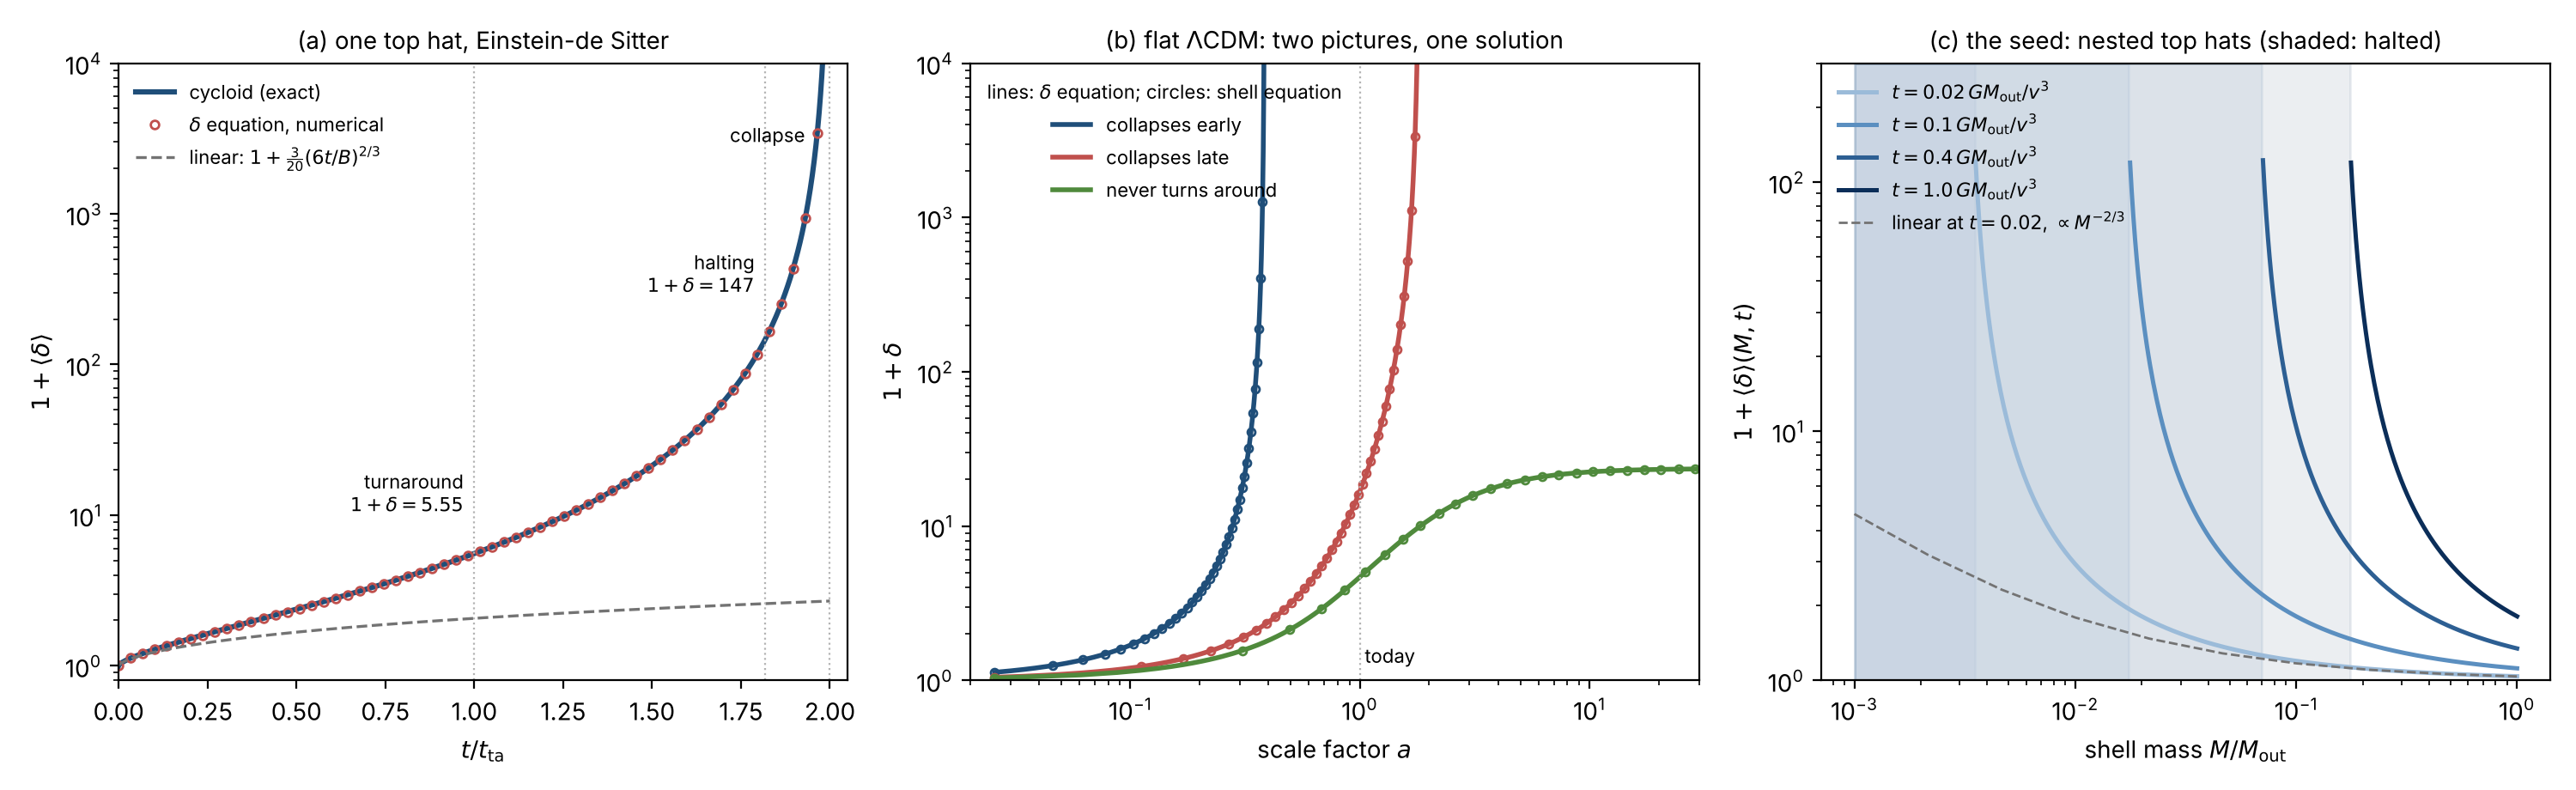
\includegraphics[width=\textwidth]{fig_tophat.png}
\caption{(a) One top hat in an Einstein--de Sitter universe: the cycloid,
Eq.~\eqref{eq:exact} (line), and the numerical solution of the $\delta$
equation, Eq.~\eqref{eq:delta} (circles), with the linear growth
(dashed). Vertical lines mark turnaround, halting and collapse.
(b) Three top hats in flat $\Lambda$CDM ($\Omega_{\rm m}=0.3$), with
initial amplitudes 3, 1.15 and 0.85 times the turnaround threshold,
Eq.~\eqref{eq:threshold}: lines from the $\delta$ equation, circles from
the shell equation, Eq.~\eqref{eq:shell}, converted with
Eq.~\eqref{eq:oneplusdelta}. The shell below the threshold never turns
around and its contrast freezes. (c) The seed of the main paper as
nested top hats: $1+\md$ against shell mass at four times,
Eq.~\eqref{eq:family}; each curve ends at the halting front,
$1+\md=147$, and the shaded regions hold the halted shells, where the
top-hat description no longer applies. The dashed line is the linear
profile $\md\propto M^{-2/3}$ at the earliest time.}
\label{fig:tophat}
\end{figure}

\section{Summary}

\begin{itemize}
\item The nonlinear equation for the density contrast of a top hat,
Eq.~\eqref{eq:delta}, is Newton's equation for the radius of its edge,
Eq.~\eqref{eq:shell}, rewritten with
$1+\delta\propto(a/R)^{3}$ (Sect.~\ref{sec:derivation}). The
cosmological constant cancels between shell and background and enters
only through $H(t)$ and $\Omega_{\rm m}(t)$.
\item In EdS the cycloid is its exact solution, Eq.~\eqref{eq:exact},
the same for every mass and energy; its linear limit is the growing mode
$\md\propto a$.
\item The mean density of our seed is this solution, one copy per shell,
shifted in time by $t_{\rm ta}\propto M$: the seed is a self-similar
family of nested top hats, with $1+\md=5.55$ at turnaround and 147 at
the halting front.
\item The density picture holds only until shells cross; in our model
that is where the front halts them. Extensions of Eq.~\eqref{eq:delta}
to clustering dark energy, shear or vorticity
\citep{DelPopolo2013,Herrera2019} add physics that a top hat in
$\Lambda$CDM does not have.
\end{itemize}

\begin{thebibliography}{99}
\bibitem[Del Popolo et al.(2013)]{DelPopolo2013} Del Popolo, A., Pace, F., \& Lima, J.~A.~S. 2013, MNRAS, 430, 628
\bibitem[Fosalba \& Gazta\~naga(1998)]{Fosalba1998} Fosalba, P., \& Gazta\~naga, E. 1998, MNRAS, 301, 503
\bibitem[Gunn \& Gott(1972)]{Gunn1972} Gunn, J.~E., \& Gott, J.~R. 1972, ApJ, 176, 1
\bibitem[Herrera et al.(2019)]{Herrera2019} Herrera, D., Waga, I., \& Jor\'as, S.~E. 2019, arXiv:1906.04326
\bibitem[Pavlidou \& Tomaras(2014)]{Pavlidou2014} Pavlidou, V., \& Tomaras, T.~N. 2014, JCAP, 09, 020
\bibitem[Peebles(1980)]{Peebles1980} Peebles, P.~J.~E. 1980, The Large-Scale Structure of the Universe (Princeton: Princeton University Press)
\end{thebibliography}

\appendix
\section{Code}
The script \texttt{code/tophat.py} (numpy, scipy, matplotlib) performs the
three checks of this note and draws Fig.~\ref{fig:tophat}; its output is
in \texttt{code/tophat\_output.txt}.
\lstinputlisting{code/tophat.py}

\end{document}
